\documentclass[12pt,addpoints]{exam}
\usepackage{amsmath, amssymb, amsthm, enumerate, graphicx}
\usepackage[usenames,dvipsnames]{color}
\usepackage{todonotes}
\usepackage{bm}
\usepackage[colorlinks=true,urlcolor=blue]{hyperref}
\usepackage{geometry}
\geometry{margin=1in}
\usepackage{float}
\usepackage{graphics}
\setlength{\marginparwidth}{2.15cm}
\usepackage{booktabs}
\usepackage{enumitem}
\usepackage{epsfig}
\usepackage{setspace}
\usepackage{parskip}
\usepackage[normalem]{ulem}
\usepackage{tikz}
\usetikzlibrary{positioning, arrows, automata}
\usepackage{pgfplots}
\usepgfplotslibrary{fillbetween}
\usepackage[font=scriptsize]{subcaption}
\usepackage{float}
\usepackage{algorithmicx}
\usepackage[noend]{algpseudocode}
\usepackage{environ}
\usepackage{bbm}
\usepackage{graphicx}
\usepackage{titling}
\usepackage{url}
\usepackage{xcolor}
\usepackage{lipsum}
\usepackage{lastpage}
\usepackage[colorlinks=true,urlcolor=blue]{hyperref}
\usepackage{multicol}
\usepackage{tabularx}
\usepackage{comment}
\usepackage{amsmath}
\usepackage{nicefrac}
\usepackage[tableposition=top]{caption}
\usepackage[many]{tcolorbox}
\usepackage{colortbl}
\usepackage{array}
\usepackage{multirow}
\usepackage{listings}
\usepackage{color}
\usepackage{adjustbox}
\usepackage{wasysym} % For \CIRCLE
\usepackage{cancel} % For \xcancel

\pgfplotsset{compat=1.16}


\definecolor{dkgreen}{rgb}{0,0.6,0}
\definecolor{gray}{rgb}{0.5,0.5,0.5}
\definecolor{mauve}{rgb}{0.58,0,0.82}

\lstset{frame=tb,
  language=Python,
  aboveskip=3mm,
  belowskip=3mm,
  showstringspaces=false,
  columns=flexible,
  basicstyle={\small\ttfamily},
  numbers=none,
  numberstyle=\tiny\color{gray},
  keywordstyle=\color{blue},
  commentstyle=\color{dkgreen},
  stringstyle=\color{mauve},
  breaklines=true,
  breakatwhitespace=true,
  tabsize=3
}


\newcommand{\class}{10-301/601 Machine Learning}
\newcommand{\term}{Spring 2023}
\newcommand{\examnum}{Exam 2}
\newcommand{\examdate}{11/09/2023}
\newcommand{\timelimit}{120 minutes}
\newcommand{\argmax}{\operatornamewithlimits{arg\,max}}
\newcommand{\argmin}{\operatornamewithlimits{arg\,min}}

% Instead of lines, use blank space.
%\renewcommand{\fillwithlines}[1]{\vspace{#1}}

\def\x{\mathbf x}
\def\y{\mathbf y}
\def\w{\mathbf w}
\def\v{\mathbf v}
\def\E{\mathbb E}
\def\V{\mathbb V}
\def\a{\mathbf a}
\def\z{\mathbf z}

\newcommand\MyBox[1]{%
  \fbox{\parbox[c][1.7cm][c]{1.7cm}{\centering #1}}%
}
\newcommand\MyVBox[1]{%
  \parbox[c][1.7cm][c]{2.5cm}{\centering\bfseries #1}%
}  
\newcommand\MyHBox[2][\dimexpr1.7cm+2\fboxsep\relax]{%
  \parbox[c][1cm][c]{#1}{\centering\bfseries #2}%
}  
\newcommand\MyTBox[3]{
  \MyVBox{#1}\MyBox{#2}
  \MyBox{#3}\par
}


\newcommand{\pts}[1]{(#1 points)}

% SOLUTION environment
\newenvironment{soln}{\leavevmode\color{red}\ignorespaces }{}

% QUESTION AUTHORS environment
\newenvironment{qauthor}{\leavevmode\color{blue}\ignorespaces }{}

% Question tester comment environment
\newenvironment{qtester}{\leavevmode\color{green}\ignorespaces}{}

% TO ONLY SHOW HOMEWORK QUESTIONS, include following (else comment out):
   % \RenewEnviron{soln}{}
   \RenewEnviron{qauthor}{}
  \RenewEnviron{qtester}{}

\newcommand{\norm}[1]{\lVert #1 \rVert}
\newcommand{\st}{\mathrm{s.t.}}

\makeatletter
\newcommand{\removelatexerror}{\let\@latex@error\@gobble}
\makeatother

\setlength\linefillheight{.35in}

%%%%%%%%%%%%%%%%%%%%%%%%%%%%%%%%%%%%%%%%%%
% Custom commands                        %
%%%%%%%%%%%%%%%%%%%%%%%%%%%%%%%%%%%%%%%%%%

% First argument is width, second argument is label.
\newcommand{\blankforFITB}[2]{\underline{\hspace{#1}#2\hspace{#1}}}

\newcommand{\vc}[1]{\boldsymbol{#1}}

\newcommand{\fpartial}[2]{\frac{\partial #1}{\partial #2}}
\newcommand{\adj}[1]{\frac{\partial J}{\partial #1}}
\newcommand{\chain}[2]{\adj{#2} = \adj{#1}\frac{\partial #1}{\partial #2}}

% mathcal
\newcommand{\Ac}{\mathcal{A}}
\newcommand{\Bc}{\mathcal{B}}
\newcommand{\Cc}{\mathcal{C}}
\newcommand{\Dc}{\mathcal{D}}
\newcommand{\Ec}{\mathcal{E}}
\newcommand{\Fc}{\mathcal{F}}
\newcommand{\Gc}{\mathcal{G}}
\newcommand{\Hc}{\mathcal{H}}
\newcommand{\Ic}{\mathcal{I}}
\newcommand{\Jc}{\mathcal{J}}
\newcommand{\Kc}{\mathcal{K}}
\newcommand{\Lc}{\mathcal{L}}
\newcommand{\Mc}{\mathcal{M}}
\newcommand{\Nc}{\mathcal{N}}
\newcommand{\Oc}{\mathcal{O}}
\newcommand{\Pc}{\mathcal{P}}
\newcommand{\Qc}{\mathcal{Q}}
\newcommand{\Rc}{\mathcal{R}}
\newcommand{\Sc}{\mathcal{S}}
\newcommand{\Tc}{\mathcal{T}}
\newcommand{\Uc}{\mathcal{U}}
\newcommand{\Vc}{\mathcal{V}}
\newcommand{\Wc}{\mathcal{W}}
\newcommand{\Xc}{\mathcal{X}}
\newcommand{\Yc}{\mathcal{Y}}
\newcommand{\Zc}{\mathcal{Z}}

% mathbb
\newcommand{\Ab}{\mathbb{A}}
\newcommand{\Bb}{\mathbb{B}}
\newcommand{\Cb}{\mathbb{C}}
\newcommand{\Db}{\mathbb{D}}
\newcommand{\Eb}{\mathbb{E}}
\newcommand{\Fb}{\mathbb{F}}
\newcommand{\Gb}{\mathbb{G}}
\newcommand{\Hb}{\mathbb{H}}
\newcommand{\Ib}{\mathbb{I}}
\newcommand{\Jb}{\mathbb{J}}
\newcommand{\Kb}{\mathbb{K}}
\newcommand{\Lb}{\mathbb{L}}
\newcommand{\Mb}{\mathbb{M}}
\newcommand{\Nb}{\mathbb{N}}
\newcommand{\Ob}{\mathbb{O}}
\newcommand{\Pb}{\mathbb{P}}
\newcommand{\Qb}{\mathbb{Q}}
\newcommand{\Rb}{\mathbb{R}}
\newcommand{\Sb}{\mathbb{S}}
\newcommand{\Tb}{\mathbb{T}}
\newcommand{\Ub}{\mathbb{U}}
\newcommand{\Vb}{\mathbb{V}}
\newcommand{\Wb}{\mathbb{W}}
\newcommand{\Xb}{\mathbb{X}}
\newcommand{\Yb}{\mathbb{Y}}
\newcommand{\Zb}{\mathbb{Z}}

% mathbf lowercase
\newcommand{\av}{\mathbf{a}}
\newcommand{\bv}{\mathbf{b}}
\newcommand{\cv}{\mathbf{c}}
\newcommand{\dv}{\mathbf{d}}
\newcommand{\ev}{\mathbf{e}}
\newcommand{\fv}{\mathbf{f}}
\newcommand{\gv}{\mathbf{g}}
\newcommand{\hv}{\mathbf{h}}
\newcommand{\iv}{\mathbf{i}}
\newcommand{\jv}{\mathbf{j}}
\newcommand{\kv}{\mathbf{k}}
\newcommand{\lv}{\mathbf{l}}
\newcommand{\mv}{\mathbf{m}}
\newcommand{\nv}{\mathbf{n}}
\newcommand{\ov}{\mathbf{o}}
\newcommand{\pv}{\mathbf{p}}
\newcommand{\qv}{\mathbf{q}}
\newcommand{\rv}{\mathbf{r}}
\newcommand{\sv}{\mathbf{s}}
\newcommand{\tv}{\mathbf{t}}
\newcommand{\uv}{\mathbf{u}}
\newcommand{\vv}{\mathbf{v}}
\newcommand{\wv}{\mathbf{w}}
\newcommand{\xv}{\mathbf{x}}
\newcommand{\yv}{\mathbf{y}}
\newcommand{\zv}{\mathbf{z}}

% mathbf uppercase
\newcommand{\Av}{\mathbf{A}}
\newcommand{\Bv}{\mathbf{B}}
\newcommand{\Cv}{\mathbf{C}}
\newcommand{\Dv}{\mathbf{D}}
\newcommand{\Ev}{\mathbf{E}}
\newcommand{\Fv}{\mathbf{F}}
\newcommand{\Gv}{\mathbf{G}}
\newcommand{\Hv}{\mathbf{H}}
\newcommand{\Iv}{\mathbf{I}}
\newcommand{\Jv}{\mathbf{J}}
\newcommand{\Kv}{\mathbf{K}}
\newcommand{\Lv}{\mathbf{L}}
\newcommand{\Mv}{\mathbf{M}}
\newcommand{\Nv}{\mathbf{N}}
\newcommand{\Ov}{\mathbf{O}}
\newcommand{\Pv}{\mathbf{P}}
\newcommand{\Qv}{\mathbf{Q}}
\newcommand{\Rv}{\mathbf{R}}
\newcommand{\Sv}{\mathbf{S}}
\newcommand{\Tv}{\mathbf{T}}
\newcommand{\Uv}{\mathbf{U}}
\newcommand{\Vv}{\mathbf{V}}
\newcommand{\Wv}{\mathbf{W}}
\newcommand{\Xv}{\mathbf{X}}
\newcommand{\Yv}{\mathbf{Y}}
\newcommand{\Zv}{\mathbf{Z}}

% bold greek lowercase
\newcommand{\alphav     }{\boldsymbol \alpha     }
\newcommand{\betav      }{\boldsymbol \beta      }
\newcommand{\gammav     }{\boldsymbol \gamma     }
\newcommand{\deltav     }{\boldsymbol \delta     }
\newcommand{\epsilonv   }{\boldsymbol \epsilon   }
\newcommand{\varepsilonv}{\boldsymbol \varepsilon}
\newcommand{\zetav      }{\boldsymbol \zeta      }
\newcommand{\etav       }{\boldsymbol \eta       }
\newcommand{\thetav     }{\boldsymbol \theta     }
\newcommand{\varthetav  }{\boldsymbol \vartheta  }
\newcommand{\iotav      }{\boldsymbol \iota      }
\newcommand{\kappav     }{\boldsymbol \kappa     }
\newcommand{\varkappav  }{\boldsymbol \varkappa  }
\newcommand{\lambdav    }{\boldsymbol \lambda    }
\newcommand{\muv        }{\boldsymbol \mu        }
\newcommand{\nuv        }{\boldsymbol \nu        }
\newcommand{\xiv        }{\boldsymbol \xi        }
\newcommand{\omicronv   }{\boldsymbol \omicron   }
\newcommand{\piv        }{\boldsymbol \pi        }
\newcommand{\varpiv     }{\boldsymbol \varpi     }
\newcommand{\rhov       }{\boldsymbol \rho       }
\newcommand{\varrhov    }{\boldsymbol \varrho    }
\newcommand{\sigmav     }{\boldsymbol \sigma     }
\newcommand{\varsigmav  }{\boldsymbol \varsigma  }
\newcommand{\tauv       }{\boldsymbol \tau       }
\newcommand{\upsilonv   }{\boldsymbol \upsilon   }
\newcommand{\phiv       }{\boldsymbol \phi       }
\newcommand{\varphiv    }{\boldsymbol \varphi    }
\newcommand{\chiv       }{\boldsymbol \chi       }
\newcommand{\psiv       }{\boldsymbol \psi       }
\newcommand{\omegav     }{\boldsymbol \omega     }

% bold greek uppercase
\newcommand{\Gammav     }{\boldsymbol \Gamma     }
\newcommand{\Deltav     }{\boldsymbol \Delta     }
\newcommand{\Thetav     }{\boldsymbol \Theta     }
\newcommand{\Lambdav    }{\boldsymbol \Lambda    }
\newcommand{\Xiv        }{\boldsymbol \Xi        }
\newcommand{\Piv        }{\boldsymbol \Pi        }
\newcommand{\Sigmav     }{\boldsymbol \Sigma     }
\newcommand{\Upsilonv   }{\boldsymbol \Upsilon   }
\newcommand{\Phiv       }{\boldsymbol \Phi       }
\newcommand{\Psiv       }{\boldsymbol \Psi       }
\newcommand{\Omegav     }{\boldsymbol \Omega     }


% Abhi messing around with examdoc
\qformat{\textbf{{\Large \thequestion \; \; \thequestiontitle \ (\totalpoints \ points)}} \hfill}
\renewcommand{\thequestion}{\arabic{question}}
\renewcommand{\questionlabel}{\thequestion.}

\renewcommand{\thepartno}{\arabic{partno}}
\renewcommand{\partlabel}{\thepartno.}
\renewcommand{\partshook}{\setlength{\leftmargin}{0pt}}

\renewcommand{\thesubpart}{\alph{subpart}}
\renewcommand{\subpartlabel}{(\thesubpart)}

\renewcommand{\thesubsubpart}{\roman{subsubpart}}
\renewcommand{\subsubpartlabel}{\thesubsubpart.}

% copied from stack overflow, as all good things are
\newcommand\invisiblesection[1]{%
  \refstepcounter{section}%
  \addcontentsline{toc}{section}{\protect\numberline{\thesection}#1}%
  \sectionmark{#1}}

% quite possibly the worst workaround i have made for this class
\newcommand{\sectionquestion}[1]{
\titledquestion{#1}
\invisiblesection{#1}
~\vspace{-1em}
}

% hack for question numbers in table
\usepackage{regexpatch}
\makeatletter
\xpatchcmd*\@multicolumntable{|c|c}{|l|c}{}{}
\xpatchcmd\questions{\def\@currentlabel{\thequestiontitle}}{\def\@currentlabel{\thequestion. \thequestiontitle}}{}{}
\makeatother


\begin{document}

\begin{soln}{\huge \bf Solutions}\end{soln}

\newcommand{\toreplace}[1]{#1}
\renewcommand{\toreplace}[1]{\underline{\hspace{10em}}}
\renewcommand{\toreplace}[1]{\hphantom{\hspace{5em}}}

% Default to an empty tags environ.
\NewEnviron{tags}{}{}

\pagestyle{head}
\firstpageheader{}{}{}
\runningheader{\class}{\examnum\ - Page \thepage\ of \numpages}{\toreplace{andrewID} - \toreplace{examNumber}}
\runningheadrule

\noindent
\begin{tabular*}{\textwidth}{l @{\extracolsep{3cm}} r @{\extracolsep{6pt}} l}
\textbf{\class} & \textbf{Name:} & {Ran Tao}\\
\textbf{\term} &  \textbf{Andrew ID:} & {rtao2} \\
\textbf{\examnum} & & {\toreplace{roomNumber}}\\
\textbf{\examdate} & & {\toreplace{seatNumber}} \\
\textbf{Time Limit: \timelimit} & & {\toreplace{examNumber}}
\end{tabular*}\\
\rule[2ex]{\textwidth}{2pt}

\textbf{Instructions:}
\begin{itemize}
    \item Verify your name and Andrew ID above. 
    \item This exam contains \numpages\ pages (including this cover page).\\
    The total number of points is \numpoints. 
    %The total number of questions is \numquestions.
    %\item You are allowed to use one page of notes
    \item Clearly mark your answers in the allocated space If you have made a mistake, cross out the invalid parts of your solution, and circle the ones which should be graded.
    \item Look over the exam first to make sure that none of the \numpages\ pages are missing. 
    \item No electronic devices may be used during the exam.
    \item Please write all answers in pen or \emph{darkly} in pencil.
    \item You have \timelimit  to complete the exam. Good luck!
\end{itemize}

\begin{center}
    \pointtable[v][questions]
\end{center}

\noindent
\rule[2ex]{\textwidth}{2pt}
\clearpage

\section*{Instructions for Specific Problem Types}

For ``Select One" questions, please fill in the appropriate bubble completely:

\begin{quote}
\textbf{Select One:} Who taught this course?
\begin{list}{}
     \item\CIRCLE{} Matt Gormley
     \item\Circle{} Marie Curie
     \item\Circle{} Noam Chomsky
\end{list}
\end{quote}

If you need to change your answer, you may cross out the previous answer and bubble in the new answer:

\begin{quote}
\textbf{Select One:} Who taught this course?
\begin{list}{}
     \item\CIRCLE{} Matt Gormley
     \item\Circle{} Marie Curie\\
     \xcancel{\CIRCLE}{} Henry Chai
\end{list}
\end{quote}


For ``Select all that apply" questions, please fill in all appropriate squares completely:

\begin{quote}
\textbf{Select all that apply:} Which are scientists?
    \begin{list}{}
    \item $\blacksquare$ Stephen Hawking 
    \item $\blacksquare$ Albert Einstein
    \item $\blacksquare$ Isaac Newton
    \item $\square$ I don't know
\end{list}
\end{quote}

Again, if you need to change your answer, you may cross out the previous answer(s) and bubble in the new answer(s):

\begin{quote}
\textbf{Select all that apply:} Which are scientists?
    \begin{list}{}
    \item $\blacksquare$ Stephen Hawking 
    \item $\blacksquare$ Albert Einstein
    \item $\blacksquare$ Isaac Newton\\
    \xcancel{$\blacksquare$} I don't know
\end{list}
\end{quote}

For questions where you must fill in a blank, please make sure your final answer is fully included in the given space. You may cross out answers or parts of answers, but the final answer must still be within the given space.

\begin{quote}
\textbf{Fill in the blank:} What is the course number?

\begin{tcolorbox}[fit,height=1cm, width=4cm, blank, borderline={1pt}{-2pt},nobeforeafter]
    \begin{center}\huge10-601\end{center}
    \end{tcolorbox}\hspace{2cm}
    \begin{tcolorbox}[fit,height=1cm, width=4cm, blank, borderline={1pt}{-2pt},nobeforeafter]
    \begin{center}\huge10-\xcancel{6}301\end{center}
    \end{tcolorbox}
\end{quote}

\clearpage
\begin{questions}
% \sectionquestion{Question Template - FOR INSTRUCTOR USE}

\textbf{Format your question types as shown below.}

\begin{parts}

\part[1] \textbf{True or False:} Input question here.
    \begin{checkboxes}
     \choice True 
     \choice False
    \end{checkboxes}
    \begin{soln}
    Input solution here.
    \end{soln}
    \begin{qauthor}
    Input (1) author name, (2) learning objective addressed, and (3) source if  adapting/reusing a question.
    \end{qauthor}

\part[1] \textbf{Select one:} Input question here
    \begin{checkboxes}
     \choice Stephen Hawking 
     \choice Albert Einstein
     \choice Isaac Newton
     \choice I don't know
    \end{checkboxes}
    \begin{soln}
    Input solution here.
    \end{soln}
    \begin{qauthor}
    Input (1) author name, (2) learning objective addressed, and (3) source if  adapting/reusing a question.
    \end{qauthor}
    
\part[1] \textbf{Select all that apply:} Input question here.
    \begin{checkboxessquare}
     \choice Stephen Hawking 
     \choice Albert Einstein
     \choice Isaac Newton
     \choice None of the above
    \end{checkboxessquare}
    \begin{soln}
    Input solution here.
    \end{soln}
    \begin{qauthor}
    Input (1) author name, (2) learning objective addressed, and (3) source if  adapting/reusing a question.
    \end{qauthor}
    
\part[1] \textbf{Fill in the blank:} \textit{Input your \underline{\hspace{8em}} here.}
    \begin{checkboxes}
     \choice money 
     \choice dignity
     \choice question
     \choice I don't know
    \end{checkboxes}
    \begin{soln}
    Input solution here.
    \end{soln}
    \begin{qauthor}
    Input (1) author name, (2) learning objective addressed, and (3) source if  adapting/reusing a question.
    \end{qauthor}
        
\part[1] \textbf{Numerical answer:} Input your question here.
    \begin{answer_box}[title=,height=1cm, width=2cm]
    \end{answer_box}
    \begin{soln}
    Input solution here.
    \end{soln}
    \begin{qauthor}
    Input (1) author name, (2) learning objective addressed, and (3) source if  adapting/reusing a question.
    \end{qauthor}

    
\part[1] \textbf{Ordering:}  Input your question here. 
\textit{Select the correct ordering of the items below by numbering them from 1 to 3.}
    \begin{itemize}
        \item Something 
            \begin{answer_box}[title=,height=1cm, width=2cm,nobeforeafter,box align=center]
            \end{answer_box}
        \item Another thing 
            \begin{answer_box}[title=,height=1cm, width=2cm,nobeforeafter,box align=center]
            \end{answer_box}
        \item Still another
            \begin{answer_box}[title=,height=1cm, width=2cm,nobeforeafter,box align=center]
            \end{answer_box}
    \end{itemize}
    \begin{soln}
    Input solution here.
    \end{soln}
    \begin{qauthor}
    Input (1) author name, (2) learning objective addressed, and (3) source if  adapting/reusing a question.
    \end{qauthor}

\part[1] \textbf{Short answer:} Input your question here.
    \fillwithlines{8em}
    \begin{soln}
    Input solution here.
    \end{soln}
    \begin{qauthor}
    Input (1) author name, (2) learning objective addressed, and (3) source if  adapting/reusing a question.
    \end{qauthor}
    
\part[1] \textbf{Derivation:} Input your question here.
    \begin{answer_box}[title=,height=5cm, width=15cm]
    \end{answer_box}
    \begin{soln}
    Input solution here.
    \end{soln}
    \begin{qauthor}
    Input (1) author name, (2) learning objective addressed, and (3) source if  adapting/reusing a question.
    \end{qauthor}

\part[1] \textbf{Proof:} Input your question here.
    \begin{answer_box}[title=,height=5cm, width=15cm]
    \end{answer_box}
    \begin{soln}
    Input solution here.
    \end{soln}
    \begin{qauthor}
    Input (1) author name, (2) learning objective addressed, and (3) source if  adapting/reusing a question.
    \end{qauthor}

\part \textit{For questions like this one that require some preamable, you should rely on the parts environment.} Consider the function $f(x)=3x^3+2x^2+x+1$. Do NOT include points on the \textit{question}, only on the \textit{part}.
    \begin{subparts}
    \subpart[10] \textit{Here you drop in one of the question templates above, replacing the question command with the part command.} Calculate $f'(x)$.
    \addpoints
    \subpart[10] \textit{Here you drop in one of the question templates above, replacing the question command with the part command.} Calculate $f''(x)$.
    \end{subparts}

\end{parts}

% \clearpage
% \sectionquestion{F23 TA Questions Go Here!}

\begin{parts}








\part[1] Sam is training a model to classify transactions as legitimate $(y=0)$ or fraudulent $(y=1)$.
He plans to audit the transactions marked as possible fraud, but he is only able to send in $k$ transactions out of a batch of $100$ for audit due to budget constraints, even though Sam knows that exactly $40$ transactions in each batch are fraud.
Sam thus trains a probabilistic classifier (which outputs a prediction $\widehat{y} \in [0, 1]$ for every transaction) and selects the transactions with the top $k$ predicted values $\widehat{y}$ to send in from each batch.

On a given batch of transactions, Sam evaluates his model's precision and recall when selecting $k$ transactions to audit for $k \in \{10, 20, \dots, 100\}$.
Mark each of the following plots as possible or impossible plots of precision and recall for Sam's model and, if marking impossible, explain why.

\begin{subparts}
\begin{minipage}{0.3\textwidth}
    \subpart[1] \textbf{Select one:}
    
    \begin{checkboxes}
% YOUR ANSWER
% Change \choice to \CorrectChoice for the appropriate selection/selections
\choice Possible
\choice Impossible
\end{checkboxes}
\end{minipage}
\begin{minipage}{0.4\textwidth}
\begin{tikzpicture}
    \begin{axis}[% Axis labels
                 ymin=0,ymax=1,xmin=0,xmax=100,
    			 % Axis labels
        		 xlabel=$k$,
        		 ylabel=Precision/Recall,
         		 xlabel shift={-2pt},
        		 ylabel shift={-3pt},
                  title=Model A,
         		 % General appearance
		         font=\small,
		         % axis equal image=true,
		         enlargelimits=false,
		         clip=false,
		         % Grids 
        	     grid style=dotted, grid=both,
                 major grid style={white!65!black},
        		 minor grid style={white!85!black},
		 		 xtick={0,10,...,100},
        		 ytick={0,0.1,...,1.1},
         		 minor xtick={0,0.02,...,1},
		         minor ytick={0,0.02,...,1},
        		 % Legend
        		 legend style={at={(1,0)},
                 		       anchor=south east}]
        
	
    \addplot+[red,mark=asterisk,mark size=1.7,thick] table[x=Threshold,y=Precision] {figures/data/p-1.txt};
    \addlegendentry{Precision}

    \addplot+[blue,mark=square,mark size=1.7,thick] table[x=Threshold,y=Recall] {figures/data/r-1.txt};
    \addlegendentry{Recall}

    \end{axis}
\end{tikzpicture}
\end{minipage}

    \begin{tcolorbox}[fit,height=3cm, width=15cm, blank, borderline={1pt}{-2pt}]
    %solution
    \end{tcolorbox}
    \begin{soln}
    This is possible. The TP sequence is 4, 10, 18, 20, 25, 30, 40, 40, 40, 40.
    \end{soln}


\begin{minipage}{0.3\textwidth}
    \subpart[1] \textbf{Select one:}
    
    \begin{checkboxes}
% YOUR ANSWER
% Change \choice to \CorrectChoice for the appropriate selection/selections
\choice Possible
\choice Impossible
\end{checkboxes}
\end{minipage}
\begin{minipage}{0.4\textwidth}
\begin{tikzpicture}
    \begin{axis}[% Axis labels
                 ymin=0,ymax=1,xmin=0,xmax=100,
    			 % Axis labels
        		 xlabel=$k$,
        		 ylabel=Precision/Recall,
         		 xlabel shift={-2pt},
        		 ylabel shift={-3pt},
                  title=Model B,
         		 % General appearance
		         font=\small,
		         % axis equal image=true,
		         enlargelimits=false,
		         clip=false,
		         % Grids 
        	     grid style=dotted, grid=both,
                 major grid style={white!65!black},
        		 minor grid style={white!85!black},
		 		 xtick={0,10,...,100},
        		 ytick={0,0.1,...,1.1},
         		 minor xtick={0,0.02,...,1},
		         minor ytick={0,0.02,...,1},
        		 % Legend
        		 legend style={at={(1,0)},
                 		       anchor=south east}]
        
	
    \addplot+[red,mark=asterisk,mark size=1.7,thick] table[x=Threshold,y=Precision] {figures/data/p-2.txt};
    \addlegendentry{Precision}

    \addplot+[blue,mark=square,mark size=1.7,thick] table[x=Threshold,y=Recall] {figures/data/r-2.txt};
    \addlegendentry{Recall}

    \end{axis}
\end{tikzpicture}
\end{minipage}

    \begin{tcolorbox}[fit,height=3cm, width=15cm, blank, borderline={1pt}{-2pt}]
    %solution
    \end{tcolorbox}
    \begin{soln}
    The TP sequence is 10, 20, 24, 30, 36, 36, 28, 36, 36, 40. Note that TP decreasing is not possible, so this is impossible. This can be more easily observed from the graph by noting that recall decreases.
    \end{soln}


\end{subparts}

    \begin{qauthor}
    Abhi, Precision/Recall content that does not yet have learning objectives
    \end{qauthor}





 
\end{parts}

% \sectionquestion{F23 TA Questions Go Here!} 

\begin{parts}


\part[2] \textbf{Short answer:} Suppose we have n data points $\{x_i,y_i\}_{i=1}^n$, $x_i, y_i \in \mathbb{R}$. Assume that these points were sampled from some distribution $\mathcal{P}$, which is unknown. You decide to fit a linear regression model as $\hat{y} = w_1 x + w_0$. However, since these points were sampled at random, as the sample changes, the weights obtained by training a linear regression model on the sample will change as well. We are interested in calculating the variance in the parameters $w_1,w_0$, as we get different samples. Provide an algorithm to do so using bootstrapping.
    \fillwithlines{10em}
    \begin{soln}
    For some iterations $t$, sample $n$ points from the initial set of points with replacement using bootstrapping, compute $w_1, w_0$ using these points for each $t$ and then take the variance across the $t$ iterations. 
    \end{soln}
    \begin{qauthor}
    Pranit Bootstrapping
    \end{qauthor}

\part Each of the following descriptions describes one step of an optimization algorithm. Select the appropriate algorithm name, or indicate that none apply.
\begin{subparts}
    \subpart[1] \textbf{Select one:} Using one dimension of the training data (or ``coordinate''), optimize all parameters.
    \begin{checkboxes}
     \choice Coordinate descent
     \choice Block coordinate descent
     \choice Neither
    \end{checkboxes}
    \begin{soln}
    Neither.
    \end{soln}

    \subpart[1] \textbf{Select one:} Fix all but one parameter (or ``coordinate''), and optimize the remaining parameter.
    \begin{checkboxes}
     \choice Coordinate descent
     \choice Block coordinate descent
     \choice Neither
    \end{checkboxes}
    \begin{soln}
    Coordinate descent
    \end{soln}

    \subpart[1] \textbf{Select one:} Using one subset of dimensions of the training data (or ``block of coordinates''), optimize all parameters.
    \begin{checkboxes}
     \choice Coordinate descent
     \choice Block coordinate descent
     \choice Neither
    \end{checkboxes}
    \begin{soln}
    Neither.
    \end{soln}

    \subpart[1] \textbf{Select one:} Fix all but one set of parameters (or ``block of coordinates''), and optimize the remaining parameters.
    \begin{checkboxes}
     \choice Coordinate descent
     \choice Block coordinate descent
     \choice Neither
    \end{checkboxes}
    \begin{soln}
    Block coordinate descent
    \end{soln}
\end{subparts}
    \begin{qauthor}
    Abhi. K-Means

    Distinguish between coordinate descent and block coordinate descent
    \end{qauthor}

 


\part[1] Which of the following are key assumptions of PCA?
{\checkboxchar{$\Box$} \checkedchar{$\blacksquare$}
\begin{checkboxes}
    \choice The data exists in a low k-dimensional subspace 
    \choice The features of the data are not correlated or have low correlation
    \choice The features have a linear relationship
    \choice The data is standardized
    \choice None of the above   
\end{checkboxes}}

\begin{soln}
    A,C,D
\end{soln}
\begin{qauthor}
    Tara, PCA
\end{qauthor}

\begin{qtester}
Note that some presentations of standard PCA require mean-centered data but not standardized data.
\end{qtester}


\part Recall that K-Means searches for $k$ centroids $c_z; z\in \{1,\dots ,k\}$ for $n$ data points $\{x_1, \dots , x_n \}$ which minimize the Euclidean distance for the data points to the centroids. 
\begin{subparts}
    

    \subpart[2]What is the objective function of K-Means?\\
    You can denote the Euclidean distance between two points $a$ and $b$ as $\|a-b\|_2^2$
    

    \begin{tcolorbox}[fit,height=3cm, width=15cm, blank, borderline={1pt}{-2pt}]
    \begin{soln}
    $$J(c,z) = \sum_{i=1}^n  \|x^{(i)} - c_z\|_2$$
    \end{soln}
    \end{tcolorbox}


\subpart[2] Why is random initialization not guaranteed to converge to the optimal clustering.

\fillwithlines{7em}

\begin{soln}
    The objective function of K-Means is non-convex. The random initialization method can result in the algorithm getting stuck at a local minima if two or more centroids are initialized in the same optimal cluster.
\end{soln}
\begin{qauthor}
        Tara, K-Means Define an objective function of K-Means which gives rise to a good clustering
\end{qauthor}

\begin{qtester}
Euclidean distance should be replaced with squared Euclidean distance in both places it appears in the question, right?

Part (b) seems potentially too open-ended, and you might get better answers by not asking them to try to relate it to the objective function written above.
\end{qtester}

\end{subparts}

\part[2] \textbf{True or False:} If we use the random subspace method with $k=\frac{1}{2}d$ where $d$ is the dimension of the data, then the time complexity of classification \textit{(not the big-O)} for KNN is half of the original time complexity.

\begin{checkboxes}
    \choice True
    \choice False
\end{checkboxes}

\fillwithlines{5em}
\begin{soln}
    True, the original time complexity of KNN is $nd$, with the Random subspace method 
\end{soln}

\begin{qtester}
    I'm not sure if we can, but if possible we might be able to reword/formalize this. We should also potentially state we want the naive algorithm for KNN, as we presented 2 in class.
\end{qtester}

\part Consider an HMM with two states $S_1$ and $S_2$ and two possible observations $O_1$ and $O_2$. The state transition matrix is given by
$$A = \begin{pmatrix}
0.6 & 0.4 \\
0.3 & 0.7
\end{pmatrix}$$ and the observation matrix is given by
$$B = \begin{pmatrix}
0.2 & 0.8 \\
0.9 & 0.1
\end{pmatrix}$$ You may assume that the initial state probabilities are uniform, i.e., $\pi(S_1)=\pi(S_2)=0.5$.

    \begin{subparts}
    \subpart[1] Run the forward algorithm to compute the  probabilities $\alpha_1(S_1), \alpha_1(S_2)$, $\alpha_2(S_1), \alpha_2(S_2)$ given the observation sequence $O=O_1 O_2$.
    \addpoints
    \subpart[1] Assume the backward algorithm is similarly already run for you. Can you explain how the above forward-backward algorithm can be interpreted as a message-passing algorithm? Show the message passing equations (in terms of variables) for computing the messages. 
    \addpoints
    \end{subparts}
    \begin{soln}
        \begin{enumerate}
            \item Using the backward algorithm, we can compute the marginal probabilities $P(S_t|O)$ for $t=1$ and $t=2$ as follows:
            \begin{itemize}
                \item Forward algorithm:
                    \begin{align*}
                    \alpha_1(S_1) &= b_{11} \cdot \pi_{S_1} = 0.2 \cdot 0.5 = 0.1\\
                    \alpha_1(S_2) &= b_{21} \cdot \pi_{S_2} = 0.9 \cdot 0.5 = 0.45\\
                    \alpha_2(S_1) &= \sum_{i=1}^2 \alpha_1(S_i) \cdot a_{i1} \cdot b_{1O_2} = (0.1 \cdot 0.6 \cdot 0.8) + (0.45 \cdot 0.3 \cdot 0.1) = 0.042\\
                    \alpha_2(S_2) &= \sum_{i=1}^2 \alpha_1(S_i) \cdot a_{i2} \cdot b_{2O_2} = (0.1 \cdot 0.4 \cdot 0.1) + (0.45 \cdot 0.7 \cdot 0.1) = 0.075
                    \end{align*}
            \end{itemize}
            \item The message-passing equations for the forward-backward algorithm can be written as follows:
            \begin{itemize}
                \item Forward Messages:
                \begin{align}
                \alpha_t(j) &= P(O_1, O_2, \ldots, O_t, q_t = S_j | \lambda) \
                &= \sum_{i=1}^2 \alpha_{t-1}(i) \cdot a_{ij} \cdot b_{j}(O_t)
                \end{align}
                \item Backward Messages:
                \begin{align}
                \beta_t(i) &= P(O_{t+1}, O_{t+2}, \ldots, O_T | q_t = S_i, \lambda) \
                &= \sum_{j=1}^2 a_{ij} \cdot b_j(O_{t+1}) \cdot \beta_{t+1}(j)
                \end{align}
            \end{itemize}
            \item 
        \end{enumerate}
    \end{soln}
    \begin{qauthor}
        Yash, HMM
    \end{qauthor}

\end{parts}

% \clearpage
\sectionquestion{CNNs \& RNNs}

\begin{parts}

\part For this question, you will consider the following kernel: 

\begin{center}
    \begin{tabular}{ |c|c|c| } 
     \hline
     -1 & -1 & -1 \\ \hline
     -1 & 1 & 1 \\ \hline
     -1 & 1 & 1 \\ \hline
    \end{tabular}
\end{center}

\begin{subparts}
    \subpart[1] \textbf{Numerical answer:} What is the output of convolving this kernel with the following matrix?

    \begin{center}
        \begin{tabular}{ |c|c|c| } 
         \hline
         4 & 2 & -1 \\ \hline
         0 & 3 & -1 \\ \hline
         1 & -1 & 3 \\ \hline
        \end{tabular}
    \end{center}
    
    \begin{tcolorbox}[fit,height=1cm, width=2cm, blank, borderline={1pt}{-2pt}]
        \begin{soln}
            -2
        \end{soln}
    \end{tcolorbox}
    
    \subpart[1] \textbf{Short answer:} Using \textbf{two or fewer words}, describe what feature the kernel above would detect in an image. \textbf{Hint:} focus on what shapes/patterns in an image would have the greatest magnitude when convolved with this kernel. 
    \fillwithlines{4em}
    \begin{soln}
        Corners
    \end{soln}
\end{subparts}
\begin{qauthor}
    Henry
\end{qauthor}

\part Suppose you are learning a CNN where the first convolutional layer takes color images as inputs, represented as 3 10$\times$10 channels. This layer uses 5$\times$5 kernels \emph{with no bias term} and outputs a single channel. It also uses a padding of 2 and a stride of 3. 

\begin{subparts}
    \subpart[1] \textbf{Numerical answer:} How many learnable parameters does this convolutional layer have?
    \begin{tcolorbox}[fit,height=1cm, width=2cm, blank, borderline={1pt}{-2pt}]
        \begin{soln}
            $3*5*5 = 75$
        \end{soln}
    \end{tcolorbox}
    
    \subpart[1] \textbf{Numerical answer:} What is the dimensionality of the output channel?
    \begin{tcolorbox}[fit,height=1cm, width=2cm, blank, borderline={1pt}{-2pt}]
        \begin{soln}
            4$\times$4
        \end{soln}
    \end{tcolorbox}
\end{subparts}
\begin{qauthor}
    Henry
\end{qauthor}

\clearpage
\part[2] \textbf{Select all that apply:} Neural the Narwhal is trying to train a CNN with one convolutional layer followed by a fully-connected layer. Unfortunately he can't get backpropagation to run on his state-of-the-art Commodore Amiga because his model has too many parameters. Which of the following changes to his architecture \emph{could} decrease the total number of learnable parameters in Neural's CNN?
{%
    \checkboxchar{$\Box$} \checkedchar{$\blacksquare$} % change checkbox style locally
    \begin{checkboxes}
     \choice Increase the size of his kernels
     \choice Increase the stride in his convolutional layer
     \choice Add a max pooling layer between the convolutional and fully-connected layers
     \choice Add an additional convolutional layer before the fully-connected layer
     \choice None of the above
    \end{checkboxes}
}
\begin{soln}
    A, B, C and D
\end{soln}
\begin{qauthor}
    Henry 
\end{qauthor}

\part[2] \textbf{Matching:} Markov the Narwhal is trying to train a machine learning model to predict the current outdoor temperature. He has lots of different kinds of data that he could potentially train his model with. For each kind of training data listed below, select the deep learning architecture that is \emph{best} suited to work with it; each option may be used multiple times or not at all.  
\\
\begin{mdframed}[innerrightmargin=20pt]
    \begin{multicols}{2}
        \begin{enumerate}[label=(\alph*)]
            \item Fully-connected feed-forward neural network
            \item Convolutional neural network
            \item Recurrent neural network
            \item Bidirectional recurrent neural network
        \end{enumerate}
    \end{multicols}
\end{mdframed}
\begin{center}
    \begin{tabular}{r l}
        A picture of the sky outside Markov's window & \begin{tcolorbox}[fit,height=1cm, width=2cm, blank, borderline={1pt}{-2pt}]
            %solution
        \end{tcolorbox} \\
        The previous hourly temperatures for the past 10 hours & \begin{tcolorbox}[fit,height=1cm, width=2cm, blank, borderline={1pt}{-2pt}]
            %solution
        \end{tcolorbox} \\
        The current outdoor temperature at 10 nearby cities & \begin{tcolorbox}[fit,height=1cm, width=2cm, blank, borderline={1pt}{-2pt}]
            %solution
        \end{tcolorbox} \\
        A transcript of the local news's morning weather report & \begin{tcolorbox}[fit,height=1cm, width=2cm, blank, borderline={1pt}{-2pt}]
            %solution
        \end{tcolorbox}
    \end{tabular}
\end{center}
    
\begin{soln}
    (b), (c), (a), (d) (or (c)...)
\end{soln}
\begin{qauthor}
    Henry
\end{qauthor}
    
\part Let $L$ be the length of the input sequence to some RNN model.
\begin{subparts}
    \subpart[1] \textbf{Select one:} How does the number of learnable parameters in the RNN scale as $L$ increases?
    \begin{checkboxes}
        \choice $O(1)$: the number of learnable parameters does not depend on $L$
        \choice $O(\log L)$: the number of learnable parameters grows logarithmically as $L$ increases
        \choice $O(L)$: the number of learnable parameters grows linearly as $L$ increases
        \choice $O(L^2)$: the number of learnable parameters grows quadratically as $L$ increases
    \end{checkboxes}
    \begin{soln}
        A
    \end{soln}

    \subpart[1] \textbf{Select one:} How does the computational cost of a single forward pass through the RNN model scale as $L$ increases?
    \begin{checkboxes}
        \choice $O(1)$: the computational cost does not depend on $L$
        \choice $O(\log L)$: the computational cost grows logarithmically as $L$ increases
        \choice $O(L)$: the computational cost grows linearly as $L$ increases
        \choice $O(L^2)$: the computational cost grows quadratically as $L$ increases
    \end{checkboxes}
    \begin{soln}
        C
    \end{soln}
\end{subparts}
\begin{qauthor}
    Henry
\end{qauthor}

\part Recall that a bidirectional RNN is defined by the following set of equations, which also correspond to the figure on the left: 
\begin{align*}
    \vcenter{\hbox{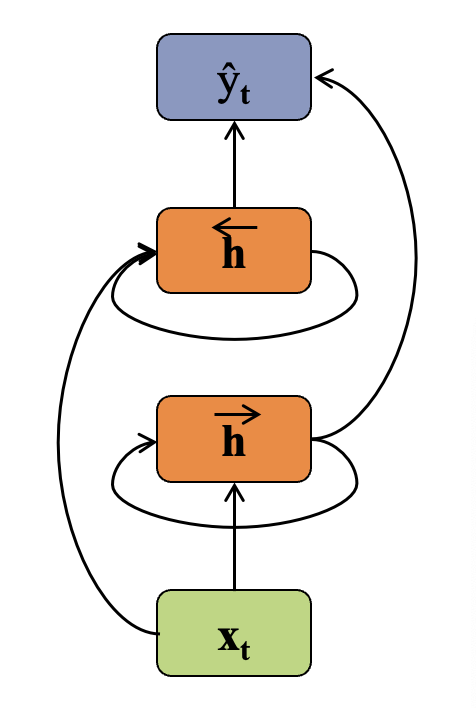
\includegraphics[width=5cm]{exam3/figures/brnn.png}}}
    \qquad
    \begin{aligned}
        \overrightarrow{\hv}_t &= \mathcal{H}(W_{x\overrightarrow{\hv}}\xv_t+W_{\overrightarrow{\hv}\overrightarrow{\hv}}\overrightarrow{\hv}_{t-1}+b_{\overrightarrow{\hv}}) \\ 
        \overleftarrow{\hv}_t &= \mathcal{H}(W_{x\overleftarrow{\hv}}\xv_t+W_{\overleftarrow{\hv}\overleftarrow{\hv}}\overleftarrow{\hv}_{t+1}+b_{\overleftarrow{\hv}}) \\ 
        \hat{y}_t &= W_{\overrightarrow{\hv}y}\overrightarrow{\hv}_t+W_{\overleftarrow{\hv}y}\overleftarrow{\hv}_t+b_y
    \end{aligned}
\end{align*}

\begin{subparts}
    \subpart[3] \textbf{Select all that apply:} Given sequences of length 3 of the form \\ $(\xv_1, y_1, \xv_2, y_2, \xv_3, y_3)$ which of the following quantities does $\overleftarrow{\hv}_2$ depend on?
    {%
    \checkboxchar{$\Box$} \checkedchar{$\blacksquare$} % change checkbox style locally
    \begin{checkboxes}
     \choice $\overrightarrow{\hv}_2$
     \choice $\xv_3$
     \choice $y_3$
     \choice $\hat{y}_3$
     \choice $\xv_1$
     \choice $W_{\overleftarrow{\hv}\overleftarrow{\hv}}$
     \choice None of the above
    \end{checkboxes}
    }
    \begin{soln}
        B, F
    \end{soln}

    \clearpage
    
    \subpart[3] \textbf{Select all that apply:} If the loss function is defined as \\ $\mathcal{L}=\sum_{t=1}^3 (y_t-\hat{y}_t)^2$, which of the following quantities does $\nicefrac{\partial \mathcal{L}}{\partial \overleftarrow{\hv}_2}$ depend on?
    {%
    \checkboxchar{$\Box$} \checkedchar{$\blacksquare$} % change checkbox style locally
    \begin{checkboxes}
     \choice $\nicefrac{\partial \mathcal{L}}{\partial \overleftarrow{\hv}_1}$
     \choice $\hat{y}_3$
     \choice $y_3$
     \choice $y_2$
     \choice $\nicefrac{\partial \mathcal{L}}{\partial W_{x\overrightarrow{\hv}}}$
     \choice $W_{\overleftarrow{\hv}y}$
     \choice None of the above
    \end{checkboxes}
    }
    \begin{soln}
        A, D, F
    \end{soln}
\end{subparts}
\begin{qauthor}
    Henry
\end{qauthor}
\end{parts}
\clearpage
\sectionquestion{Attention and Transformers}

\begin{parts}

\part[1] \textbf{True or False:} Residual (skip) connections are used in Transformers to reduce the computational inefficiency that results from increased layer connections in deep models.
    \begin{checkboxes}
        \choice True
        \choice False
    \end{checkboxes}
    \begin{soln}
    False
    \end{soln}
    \begin{qauthor}
    Siva (edited by Matt), Identify residual connection's use case.
    \end{qauthor}

\part[2] \textbf{Select all that apply:} In the context of Transformer language models, which of these statements are true regarding mask matrices?
    {%
    \checkboxchar{$\Box$} \checkedchar{$\blacksquare$} % change checkbox style locally
    \begin{checkboxes}
     \choice Mask matrices are not required in models that use attention mechanisms.
     \choice Mask matrices are only used in the training phase and not in the validation phase.
     \choice A diagonal mask matrix is used to prevent the model from accessing future tokens.
     \choice None of the above
    \end{checkboxes}
    }
    \begin{soln}
    A) False. This is incorrect as mask matrices are a crucial component in attention mechanisms, especially in Transformers.\\
    B) False. Mask matrices are used in both training and validation phases, especially in autoregressive models during validation to prevent future token visibility. \\
    C) False. Diagonal matrices are not commonly used for masking in standard Transformer models.\\
    \end{soln}
    \begin{qauthor}
    Haohui (edited by Matt), Given a description of a sequence-to-sequence machine learning task, construct the appropriate mask matrix for training a Transformer to perform the specified task
    \end{qauthor}

    \begin{qtester}
    Feedback: I'm not too much of a fan of A and B requiring them to remember exact axis layouts. C and D seem more accessible in an exam setting.
    \end{qtester}

\part[1] \textbf{Select one:} Which is the correct formula for computing  scaled dot product attention from the query $\Qv$, key $\Kv$, and value $\Vv$ matrices. Assume the dimensions of the query, key and value vectors are $d$. Assume $\text{softmax}(\cdot)$ is applied elementwise to its vector or matrix input.
\begin{checkboxes}
    \choice $\text{softmax}(\frac{(\Qv \Kv)^T}{\sqrt{d}}) \Vv$
    \choice $\text{softmax}(\frac{\Qv \Kv^T}{\sqrt{d}}) \Vv$ 
    \choice $\text{softmax}(\frac{\Qv \Vv^T}{\sqrt{d}}) \Kv$
    \choice $\text{softmax}(\frac{\Qv \Kv^T \Vv}{\sqrt{d}})$
    \choice None of the above
\end{checkboxes}
\begin{soln}
    Option B is correct.
    \end{soln}
    \begin{qauthor}
    Rakshith, Implement scaled dot-product attention in matrix form.
    \end{qauthor}
    \begin{qtester}
        High level LGTM, they should be able to shape match somewhat and use semantic meaning somewhat.
    \end{qtester}

\part[1] \textbf{True or False:} Layer normalization is used in the Transformer architecture to keep the scale of the hidden states roughly the same across layers.
    \begin{checkboxes}
     \choice True 
     \choice False
    \end{checkboxes}
    \begin{soln}
    True
    \end{soln}
    \begin{qauthor}
    Matt (inspired by Q by Rakshith), Define layer normalization and residual connections in a Transformer layer.
    \end{qauthor}

\clearpage 

\part[2] \textbf{Select all that apply:}  Why are positional embeddings necessary in the Transformer architecture for sequence modeling?
{\checkboxchar{$\Box$} \checkedchar{$\blacksquare$}
\begin{checkboxes}
    \choice To introduce randomness and enhance diversity in the model's predictions. 
    \choice To distinguish copies of the same word that appear in different parts of a sentence. %provide a potentially unique identification to each token within the sequence.
    \choice To prevent overfitting by adding noise to the input data.
    \choice To encode the order or position information of tokens in the absence of sequential operations like recurrence or convolution.
    \choice To reduce computational complexity by simplifying the token representation.
    \choice None of the above.  
\end{checkboxes}}
    \begin{soln}
    B, D only. Positional embeddings are essential in Transformers to impart sequential information to tokens within a sequence, enabling the model to discern and maintain the positional relationships between elements without relying on recurrent or convolutional operations. They help the model understand the order or position of tokens, crucial for capturing sequential dependencies in non-sequential architectures like Transformers. 
    \end{soln}
    \begin{qauthor}
    Siva (edited by Matt), Justify the use of positional embeddings in Transformers.
    \end{qauthor}
    \begin{qtester}
        Note that learned postitional encodings (e.g. embedding-based) don't necessarily guarantee uniqueness. D is solid though.

        Update: Updated the option B to reflect that the learned embeddings are not guaranteed to be unique.
    \end{qtester}


\end{parts}
\clearpage
\sectionquestion{Pre-Training, fine-tuning, in-context learning}

\begin{parts}

\begin{comment}
    
\part[2] \textbf{Short answer:} Consider a dataset with a large number of unlabelled images and a small set of labelled images. Describe a strategy that combines both supervised and unsupervised pre-training for image classification and explain why this strategy might be more effective than using either method alone.

\fillwithlines{5em}
\begin{soln}
    First apply unsupervised pre-training on the large unlabelled dataset to learn general features and representations of images. Then use supervised pre-training on the smaller labelled dataset to refine the model for specific classification tasks. Used unsupervised learning for capturing broad features without the need for labels, and supervised learning for task-specific fine-tuning, resulting in a more robust and versatile model.
\end{soln}
\begin{qauthor}
    Monica, Pretraining, Fine-tuning \& In-context Learning: Compare and contrast supervised and unsupervised pre-training
    
    Removed by Henry: a bit too open-ended imo
\end{qauthor}
\begin{qtester}
    Probably needs to be broken into parts. More direction on the strategy would also be useful. 
\end{qtester}
\end{comment}

\part[3] \textbf{Order the options:} Suppose you have a large, unlabelled dataset and a small, labelled dataset for some multi-class classification task. Given a fixed neural network architecture with many hidden layers, where the output layer is a softmax layer of the appropriate dimensionality, arrange the steps below in the order of a prototypical \emph{unsupervised} pre-training \& fine-tuning pipeline. 

Specify your answer by writing the letter corresponding to your selection for each of the five steps. \textbf{Note:} if some sequence of steps can be performed in any order, break ties in alphabetical order. 
 
\begin{enumerate}[label=\Alph*]
    \item Replace the output layer of the original neural network architecture with a sigmoid layer. 
    \item Replace the output layer of the original neural network architecture with a linear layer that has the same dimensionality as your input layer. 
    \item Optimize the weights of the entire network simultaneously using the unlabelled dataset by minimizing the reconstruction error. 
    \item Optimize the weights of the entire network simultaneously using the labelled dataset by minimizing the cross-entropy loss. 
    \item Optimize the weights of the network layerwise, starting from the input layer, using the unlabelled dataset by minimizing the reconstruction error.  
    \item Optimize the weights of the network layerwise, starting from the input layer, using the labelled dataset by minimizing the cross-entropy loss. 
    \item Initialize the weights of your network randomly.
    \item Initialize the weights of your network to the pre-trained weights. 
\end{enumerate}
\begin{comment}
\mbox{\begin{tcolorbox}[enhanced, sidebyside align=top, box align=top, height=2.5cm, width=3cm, colback=white, borderline={1pt}{-2pt} colbacktitle=black, title=Step 1]
        %solution
\end{tcolorbox}\hspace{1em}\begin{tcolorbox}[enhanced, sidebyside align=top, box align=top, height=2.5cm, width=3cm, colback=white, borderline={1pt}{-2pt} colbacktitle=black, title=Step 2]
        %solution
\end{tcolorbox}\hspace{1em}\begin{tcolorbox}[enhanced, sidebyside align=top, box align=top, height=2.5cm, width=3cm, colback=white, borderline={1pt}{-2pt} colbacktitle=black, title=Step 3]
        %solution
\end{tcolorbox}\hspace{1em}\begin{tcolorbox}[enhanced, sidebyside align=top, box align=top, height=2.5cm, width=3cm, colback=white, borderline={1pt}{-2pt} colbacktitle=black, title=Step 4]
        %solution
\end{tcolorbox}\hspace{1em}\begin{tcolorbox}[enhanced, sidebyside align=top, box align=top, height=2.5cm, width=3cm, colback=white, borderline={1pt}{-2pt} colbacktitle=black, title=Step 5]
        %solution
\end{tcolorbox}}
\end{comment}
\mbox{\begin{your_solution}[height=2.5cm, width=3cm, title=Step 1]
        %solution
\end{your_solution}\hspace{0.5em}\begin{your_solution}[height=2.5cm, width=3cm, title=Step 2]
        %solution
\end{your_solution}\hspace{0.5em}\begin{your_solution}[height=2.5cm, width=3cm, title=Step 3]
        %solution
\end{your_solution}\hspace{0.5em}\begin{your_solution}[height=2.5cm, width=3cm, title=Step 4]
        %solution
\end{your_solution}\hspace{0.5em}\begin{your_solution}[height=2.5cm, width=3cm, title=Step 5]
        %solution
\end{your_solution}}

\begin{soln}
    B - G - E - H - D
\end{soln}
\begin{qauthor}
    Henry
\end{qauthor}

\clearpage

\part[1] \textbf{Select one:} Which of the following options best describes the role of human feedback in Reinforcement Learning from Human Feedback (RLHF)?
\begin{checkboxes}
    \choice Human feedback is used to pre-train a model on general tasks before any specific training.
    \choice Human feedback is used to train a reward function for reinforcement learning. 
    \choice Human feedback is used to tune model hyperparameters.
    \choice Human feedback is used to evaluate a model after training has convereged. 
\end{checkboxes}
    
\begin{soln}
    B: RLHF uses feedback from humans to guide the training process, making it more nuanced and aligned with human values and judgments.
\end{soln}
\begin{qauthor}
    Monica, Pretraining, Fine-tuning \& In-context Learning: Define reinforcement learning from human feedback (RLHF) 

    Lightly edited by Henry
\end{qauthor}
\begin{qtester}
    LGTM
\end{qtester}

\part[2] \textbf{Select all that apply:} Given a pre-trained language model, which of the following procedures directly change the pre-trained model's weights? 
{%
    \checkboxchar{$\Box$} \checkedchar{$\blacksquare$} % change checkbox style locally
    \begin{checkboxes}
        \choice In-context Learning
        \choice Supervised Fine-tuning
        \choice Zero-shot Learning
        \choice Reinforcement Learning from Human Feedback
        \choice None of the above
    \end{checkboxes}
}
\begin{soln}
    B and D; In-context learning refers to the LLMs ability to learn from the inputs without updating any model parameters. Zero-shot learning is a form of in-context learning. 
\end{soln}
\begin{qauthor}
    Henry
\end{qauthor}

\part[2] \textbf{Short answer:} Given a pre-trained \underline{large} language model (LLM) and some amount of labelled training data, what is one reason why it might be better to perform in-context learning using the LLM rather than  fine-tune the LLM using the training dataset? 
\fillwithlines{9em}
\begin{soln}
    You don't have enough labelled data to effectively fine-tune the parameters \emph{AND} you don't have enough computational resources to perform supervised fine-tuning. 
\end{soln}
\begin{qauthor}
    Henry
\end{qauthor}

\begin{comment}
\part[2] \textbf{Short answer:}Neural The Narwhal is tasked with developing a language model for the diamond market at a startup. Faced with limited data availability, Tensor the Tiger advises improving the model's performance by fine-tuning. Which approach should Neural consider to best address this challenge?
\fillwithlines{10em}
\begin{soln}
\textbf{Solution}: Since fine-tuning typically requires a substantial amount of specific, labeled data, which is not available in this case, Neural should leverage in-context learning. This approach involves providing the language model with carefully crafted prompts and examples related to the diamond market.\\
\end{soln}
\begin{qauthor}
    Sahithya, Provide examples where in-context learning might be necessary/preferable relative to supervised fine-tuning.
    
    Removed by Henry due to ambiguity
\end{qauthor}
\begin{qtester}
        Question needs to specify what approaches the answer can be selected out of. Right now the question says Neural is going to fine-tune but Neural doesn't actually fine-tune.    
\end{qtester}
\end{comment}

\end{parts}
\clearpage
\sectionquestion{MDPs and Value/Policy Iteration}

\begin{parts}


\part Suppose we wish to learn to play the classic side-scrolling computer game Lemmings. For the first level, each state $s=(s_{ij}, s_d)$ in state space $\Sc$ contains the lemming's position ($s_{ij}$), the lemming's direction ($s_d \in \{\text{left}, \text{right}\}$). The action space is $\Ac = \{$ \texttt{continue}, \texttt{dig} $\}$. 
\begin{itemize}
    \item The \texttt{continue} action allows the lemming to walk one tile in its current direction (left or right). 
    \\
    \textit{Example:} From  $s=(s_{22}, \text{right})$ taking \texttt{continue} yields $s=(s_{23}, \text{right})$.
    
    \item Physics applies: if the direction $s_d$ leads into solid tile (brown or gray), the lemming position remains unchanged but its direction switches. 
    \\
    \textit{Example:} From $s=(s_{47}, \text{right})$ taking \texttt{continue} yields $s=(s_{47}, \text{left})$.
    
    \item Gravity applies: If the lemming is above a non-solid tile (white or blue), it will fall down one tile regardless of its direction. %\textit{Example:} if the lemming is moving right from $s_{55}$, in one turn it moves to $s_{56}$, and in two turns to $s_{46}$. 
    \\
    \textit{Example:} From $s=(s_{55}, \text{right})$ taking \texttt{continue} yields $s=(s_{56}, \text{right})$.
    \\
    \textit{Example:} From $s=(s_{56}, \text{right})$ taking any action yields $s=(s_{46}, \text{right})$.
    
    \item The \texttt{dig} action allows the lemming to move down through a dirt tile (brown). 
    Taking the \texttt{dig} action over a non-dirt tile leads to the same result as if the \texttt{continue} action were taken.
    \\
    \textit{Example:} From $s=(s_{53}, \text{left})$ taking \texttt{dig} yields $s=(s_{43}, \text{left})$.
    \\
    \textit{Example:} From $s=(s_{43}, \text{left})$ taking any action yields $s=(s_{33}, \text{left})$.
\end{itemize}
The goal tile (yellow) and the water tiles (blue) are terminal states. The reward function returns $+100$ for entering the goal tile and $-100$ for entering a water tile. Assume $\gamma = 0.9$.

    \begin{center}
        \begin{tikzpicture}
        
            % Coloring specific cells
            \foreach \i in {1,...,9} {
                \fill[gray] (\i-1,5) rectangle (\i,6); % top row
                \fill[gray] (\i-1,0) rectangle (\i,1); % bottom row  
            }
            \foreach \j in {1,...,6} {
                \fill[gray] (0,\j-1) rectangle (1,\j); % left col
                \fill[gray] (8,\j-1) rectangle (9,\j); % right col  
            }
            \foreach \i in {3,...,5} {
                \fill[brown] (\i-1,3) rectangle (\i,4); 
            }
            \foreach \i in {6,...,7} {
                \fill[brown] (\i-1,2) rectangle (\i,3); 
            }
            \fill[brown] (1,3) rectangle (2,4);
            \fill[brown] (2,3) rectangle (3,4);
            
            \fill[blue] (4,0) rectangle (5,1);
            \fill[blue] (3,0) rectangle (4,1);  
            \fill[yellow] (7,1) rectangle (8,2);
            
            \fill[gray] (7,3) rectangle (8,4);
            \fill[gray] (8,3) rectangle (9,4);

            \node at (1.5,4.5) {
\includegraphics[width=0.8cm]{figures/lemming.png}};
            
            \draw[step=1cm] (0,0) grid (9, 6);
            
            % Loop to place s_{ij} in each cell
            \foreach \i in {1,...,9} {
                \foreach \j in {1,...,6} {
                    % Places s_{ij} at the center of the cell (\i+1,\j+1)
                    \node at (\i+0.75-1,\j+0.75-1) {$s_{\j\i}$};
                }
            }
            
        \end{tikzpicture}
    \end{center}

\begin{subparts}

\subpart[1] \textbf{Numerical answer:} What is $V^*(s)$ for $s=(s_{27}, \text{right})$?
    \begin{tcolorbox}[fit,height=1cm, width=2cm, blank, borderline={1pt}{-2pt}]
    %solution
    \end{tcolorbox}
    \begin{soln}
    $+100$
    \end{soln}
    \begin{qauthor} Matt    \end{qauthor}

\clearpage
    
\subpart[1] \textbf{Numerical answer:} What is $V^*(s)$ for $s=(s_{27}, \text{left})$?
    \begin{tcolorbox}[fit,height=1cm, width=2cm, blank, borderline={1pt}{-2pt}]
    %solution
    \end{tcolorbox}
    \begin{soln}
    $0.9^2 * -100$
    \end{soln}
    \begin{qauthor} Matt    \end{qauthor}
    
\subpart[2] \textbf{Select one:} Suppose we are in a state $s=(s_{ij}, s_d)$ where $s_{ij} = s_{46}$. Is the action $a=$dig always an optimal action? \textbf{Briefly justify your answer.}
    \begin{checkboxes}
     \choice Yes
     \choice No
    \end{checkboxes}    
    \fillwithlines{8em}
    \begin{soln}
    No. If $s_d=$right, it is optimal. If $s_d=$left, it would cause the lemming to walk into the water, so $a=$continue should be chosen instead.
    \end{soln}
    \begin{qauthor} Matt    \end{qauthor}

\subpart[1] \textbf{Select one:} How many optimal policies are there for this problem?
    \begin{checkboxes}
     \choice zero
     \choice one
     \choice an integer greater than one
     \choice infinitely many
    \end{checkboxes}
    \begin{soln}
    an integer greater than one
    \end{soln}
    \begin{qauthor} Matt    \end{qauthor}

\subpart[1] \textbf{Numerical answer:} What is $Q^*(s,a)$ for $s=(s_{54}, \text{right})$ and $a=\texttt{dig}$?
    \begin{tcolorbox}[fit,height=1cm, width=2cm, blank, borderline={1pt}{-2pt}]
    %solution
    \end{tcolorbox}
    \begin{soln}
    $0.9^3 * -100 = -72.9$
    \end{soln}
    \begin{qauthor} Matt    \end{qauthor}

\subpart[1] \textbf{Select one:} Does this environment have stochastic transitions or deterministic transitions?
    \begin{checkboxes}
     \choice stochastic transitions
     \choice deterministic transitions
    \end{checkboxes}
    \begin{soln}
    deterministic transitions
    \end{soln}
    \begin{qauthor} Matt    \end{qauthor}
    
    
\end{subparts}


\part[2] \textbf{Select all that apply:} Which of the following is true of a Markov decision process (MDP)?
    {%
    \checkboxchar{$\Box$} \checkedchar{$\blacksquare$} % change checkbox style locally
    \begin{checkboxes}
     \choice An MDP defines one way that the state, action, reward tuples are gathered for reinforcement learning.
     \choice The components of an MDP include a state space, action space, transition probabilities, reward function, and policy.
     \choice Every state/action space of finite size consists of exactly one optimal policy.
     \choice The Bellman equations are a recursive definition of the optimal policy.
     \choice None of the above
    \end{checkboxes}
    }
    \begin{soln}
    A, B
    \end{soln}
    \begin{qauthor}
    Matt
    \end{qauthor}

\part[1] \textbf{True or False:} Value iteration learns the optimal value function from which we can infer the optimal policy. By contrast, policy iteration learns the optimal policy from which we \emph{cannot} infer the optimal value function.
    \begin{checkboxes}
     \choice True 
     \choice False
    \end{checkboxes}
    \begin{soln}
    False, we can infer the optimal value function from the optimal policy.
    \end{soln}
    \begin{qauthor}
    Matt
    \end{qauthor}


\end{parts}
\clearpage
\sectionquestion{Q-Learning and Deep RL}

\begin{parts}

\part Bocchi and Dora are both running tabular Q-learning on the same environment with unknown nondeterministic transitions. 
The two use the exact same parameters, except the value for $\epsilon$ in their $\epsilon$-greedy action selection (i.e. choose a random action with probability $\epsilon$, and a greedy action with probability $(1-\epsilon)$).
Since Bocchi does not like exploring, she sets $\epsilon = 0$. Meanwhile, Dora loves exploring so she sets $\epsilon = 1$.
%
Assume the discount factor $\gamma$ satisfies $0 \leq \gamma < 1$, rewards are finite and bounded, Q-values are initialized to zero, and learning rate $\alpha_t$ follows the schedule $\alpha_t = \frac{1}{t+1}$.

    \begin{subparts}
        \subpart[2] \textbf{Select one:} Over an arbitrarily large number of steps, is Bocchi's Q-learning algorithm guaranteed to converge to the optimal Q-value function? \textbf{Explain in one sentence.}
        \begin{checkboxes}
            \choice Yes
            \choice No
        \end{checkboxes}
        \fillwithlines{5em}
        \begin{soln}
        No, since Bocchi's algorithm isn't guaranteed to visit every state 
        \end{soln}

        \subpart[2] \textbf{Select one:} Over an arbitrarily large number of steps, is Dora's Q-learning algorthim guaranteed to converge to the optimal Q-value function?  \textbf{Explain in one sentence.}
        \begin{checkboxes}
            \choice Yes
            \choice No
        \end{checkboxes}
        \fillwithlines{5em}
        \begin{soln}
            Yes, since Dora's algorithm is guaranteed to visit every state arbitrarily many times
        \end{soln}

        \begin{comment}
        \subpart[2] \textbf{Short answer:} Why might it be preferable to set $\epsilon$ to a small non-zero constant instead of exactly $0$ or $1$?
        \fillwithlines{7em}
        \begin{soln}
            $\epsilon$-greedy strikes a balance between exploration and exploitation; it is guaranteed to converge unlike a pure greedy strategy and likely to converge faster than a pure random strategy.
        \end{soln}
        \end{comment}
        
    \end{subparts}
        

\begin{qauthor}
    Alex, Identify the conditions under which the Q-learning algorithm will converge to the true value function
\end{qauthor}

\clearpage

\part Consider a supervised online learning problem in which your goal is to minimize the number of mistakes made on a stream of examples $(\xv^{(1)}, y^{(1))}), (\xv^{(2)}, y^{(2))}), \ldots$ where $\xv^{(i)} \in \Rb^M$ and $y^{(i)} \in \{+1, -1\}$ and $y^{(i)} = c^*(\xv^{(i)})$. Assume for all $i \neq j$, $\xv^{(i)} \neq \xv^{(j)}$ and that the model is not able to view any past points after a new one arrives.

In this problem, you will recast this \textit{online learning} problem as a \textit{reinforcement learning} problem by defining your state space $\Sc$, action space $\Ac$, reward function $R(s,a)$, and transition function $\delta(s,a)$. Your goal is to learn a linear model $\hat{y}^{(i)} = h_{\thetav}(\xv^{(i)}) = \text{sign}(\thetav^T\xv^{(i)})$. 

\textbf{(For full credit, all your answers must be in terms of mathematical quantities appearing in the above paragraphs.)}

\begin{subparts}

\subpart[1] \textbf{Short answer:} What is the state at timestep $t$, i.e. $s_{t}$?
    \begin{tcolorbox}[fit,height=1cm, width=4cm, blank, borderline={1pt}{-2pt}]
    %solution
    \end{tcolorbox}
    \begin{soln}
    $\xv^{(t)}$, i.e. the $t$th feature vector
    \end{soln}
    \begin{qauthor}   Matt    \end{qauthor}

\subpart[1] \textbf{Short answer:} Define the state space, $\Sc$.
    \begin{tcolorbox}[fit,height=1.5cm, width=6cm, blank, borderline={1pt}{-2pt}]
    %solution
    \end{tcolorbox}
    \begin{soln}
    $\Rb^M$, i.e. real-valued vectors of length $M$
    \end{soln}
    \begin{qauthor}   Matt    \end{qauthor}

% \subpart[1] \textbf{Short answer:} What is the greedy action at timestep $t$, i.e. $a_{t}$?
%     \begin{tcolorbox}[fit,height=1cm, width=4cm, blank, borderline={1pt}{-2pt}]
%     %solution
%     \end{tcolorbox}
%     \begin{soln}
%     $\hat{y}^{(t)}$, i.e. the $t$th prediction
%     \end{soln}
%     \begin{qauthor}   Matt    \end{qauthor}
    
\subpart[1] \textbf{Short answer:} Define the action space, $\Ac$.
    \begin{tcolorbox}[fit,height=1.5cm, width=6cm, blank, borderline={1pt}{-2pt}]
    %solution
    \end{tcolorbox}
    \begin{soln}
    $\{+1, -1\}$, i.e. assigning a label of $+1$ or $-1$ to $y^{(i)}$
    \end{soln}
    \begin{qauthor}   Matt    \end{qauthor}
    
\subpart[1] \textbf{Short answer:} Define the reward function, $R(s, a) : \Sc \times \Ac \rightarrow \Rb$.
    \begin{tcolorbox}[fit,height=1.9cm, width=8cm, blank, borderline={1pt}{-2pt}]
    %solution
    \end{tcolorbox}
    \begin{soln}
    \begin{align*}
        R(\xv^{(t)}, a) = \begin{cases}
        1 & \text{if } y^{(t)} = a \\
        0 & \text{if } y^{(t)} \neq a 
        \end{cases}
    \end{align*}
    \end{soln}
    \begin{qauthor}   Matt    \end{qauthor}
    
\subpart[1] \textbf{Short answer:} Define the transition function, i.e. $s_{t+1} = \delta(s_t, a_t)$.
    \begin{tcolorbox}[fit,height=1.9cm, width=8cm, blank, borderline={1pt}{-2pt}]
    %solution
    \end{tcolorbox}
    \begin{soln}
    $\delta(\xv^{(t)}, \hat{y}^{(t)}) = \xv^{(t+1)}$
    \end{soln}
    \begin{qauthor}   Matt    \end{qauthor}

% \subpart[1] \textbf{Short answer:} Define the policy, $\pi(s_t) : \Sc \rightarrow \Ac$.
%     \begin{tcolorbox}[fit,height=2cm, width=8cm, blank, borderline={1pt}{-2pt}]
%     %solution
%     \end{tcolorbox}
%     \begin{soln}
%     $\pi(\xv^{(t)}) = h_{\thetav}(\xv^{(t)}) = \text{sign}(\thetav^T \xv^{(t)})$
%     \end{soln}
%     \begin{qauthor}   Matt    \end{qauthor}


\subpart[1] \textbf{Select one:} Which of the following would be the best choice to learn a policy $\pi : \Sc \rightarrow \Ac$?
    \begin{checkboxes}
     \choice value iteration
     \choice policy iteration
     \choice tabular Q-learning
     \choice deep Q-learning
    \end{checkboxes}
    \begin{soln}
    deep Q-learning
    \end{soln}
    \begin{qauthor}   Matt    \end{qauthor}

    
\end{subparts}


\end{parts}
\clearpage
\input{qs-PCA.tex}
\clearpage
\sectionquestion{$K$-Means}

\begin{parts}

\part Suppose we wish to apply $K$-Means to the unlabeled 2D dataset $\Dc = \{ \xv^{(i)} \}_{i=1}^N$ below.

\begin{center}
\begin{tikzpicture}[thick,scale=0.9, every node/.style={transform shape}]
    \begin{axis}[
        axis equal image,
        xmin=-5, xmax=5, xtick={-5,...,5},
        ymin=-3, ymax=3, ytick={-3,...,3},
        xlabel={$x_1$}, ylabel={$x_2$},
        samples=50, grid=major, minor tick num=1,
        xticklabel style={xshift=-0.1cm}]
      \addplot [
            scatter,
            only marks,
            point meta=explicit symbolic,
            scatter/classes={
                a={mark=square*,black}
            },
            nodes near coords*={$\xv^{(\pgfmathprintnumber[frac]\myvalue)}$},
            visualization depends on={\thisrow{myvalue} \as \myvalue},
        ] table [meta=label] {
            x y label myvalue
            -4 -2 a 1
            -2 -2 a 2
            -4 0 a 3
            0 0 a 4
            1 2 a 5
            3 0 a 6
            4 -1 a 7
        };
    \end{axis}
\end{tikzpicture}
\end{center}
 
We set $K=3$ and initialize the cluster centers to $\xv^{(4)}, \xv^{(5)}, \xv^{(7)}$. 
(Assume a single iteration first computes cluster assignments and then computes cluster centers.) 

\begin{subparts}

    \subpart[2] \textbf{Short answer:} What will the partitioning of the points be after the \textbf{first} iteration of $K$-Means? 

        cluster 1: \hspace{3.2cm} cluster 2:  \hspace{3.2cm} cluster 3: 
                
        \begin{tcolorbox}[fit,height=1cm, width=4.5cm, blank, borderline={1pt}{-2pt},nobeforeafter]
        %solution
        \end{tcolorbox}
        \hspace{1em}
        \begin{tcolorbox}[fit,height=1cm, width=4.5cm, blank, borderline={1pt}{-2pt},nobeforeafter]
        %solution
        \end{tcolorbox}
        \hspace{1em}        
        \begin{tcolorbox}[fit,height=1cm, width=4.5cm, blank, borderline={1pt}{-2pt},nobeforeafter]
        %solution
        \end{tcolorbox}
        
        \begin{soln}
        The rubric here should almost certainly NOT be a simple binary check of whether each cluster is correct. That is, there will probably be only a small number of wrong answers and we should group those into equivalence classes.
        
        cluster 1: $\xv^{(1)}, \xv^{(2)}, \xv^{(3)}, \xv^({4})$\\
        cluster 2: $\xv^{(5)}$\\
        cluster 3: $\xv^{(6)}, \xv^{(7)}$\\
        \end{soln}
        \begin{qauthor}
        Matt
        \end{qauthor}

    \subpart[2] \textbf{Short answer:} What will the partitioning of the points be after the \textbf{second} iteration of $K$-Means?

        cluster 1: \hspace{3.2cm} cluster 2:  \hspace{3.2cm} cluster 3: 
                
        \begin{tcolorbox}[fit,height=1cm, width=4.5cm, blank, borderline={1pt}{-2pt},nobeforeafter]
        %solution
        \end{tcolorbox}
        \hspace{1em}
        \begin{tcolorbox}[fit,height=1cm, width=4.5cm, blank, borderline={1pt}{-2pt},nobeforeafter]
        %solution
        \end{tcolorbox}
        \hspace{1em}        
        \begin{tcolorbox}[fit,height=1cm, width=4.5cm, blank, borderline={1pt}{-2pt},nobeforeafter]
        %solution
        \end{tcolorbox}
        
        \begin{soln}
        The rubric here should almost certainly NOT be a simple binary check of whether each cluster is correct. That is, there will probably be only a small number of wrong answers and we should group those into equivalence classes.

        cluster 1: $\xv^{(1)}, \xv^{(2)}, \xv^{(3)}$\\
        cluster 2: $\xv^({4}), \xv^{(5)}$\\
        cluster 3: $\xv^{(6)}, \xv^{(7)}$\\
        \end{soln}
        \begin{qauthor}
        Matt
        \end{qauthor}

    \subpart[1] \textbf{Short answer:} How many total iterations will complete before $K$-Means has converged? (We say that $K$-Means has converged if the next iteration, the cluster assignment will not change.)
        \begin{tcolorbox}[fit,height=1cm, width=4cm, blank, borderline={1pt}{-2pt}]
        %solution
        \end{tcolorbox}        
        \begin{soln}
        2
        \end{soln}
        \begin{qauthor}
        Matt
        \end{qauthor}

\end{subparts}

\part[1] \textbf{True or False:} Given a fixed set of initial cluster centers, $K$-Means \emph{always} converges to the same final cluster assignment, assuming ties in distance are always broken the same way.

    \begin{checkboxes}
     \choice True 
     \choice False
    \end{checkboxes}
    \begin{soln}
    True
    \end{soln}
    \begin{qauthor}
    Matt -- Note for future semesters: We should have labeled the points A, B, C, D,... for easier reading when grading. Also if we had one box for each point and we asked students to simply label them with cluster IDs, then we could auto-grade with Hamming loss.
    \end{qauthor}

\begin{comment}
\part[1] \textbf{True or False:} $K$-Means++ initialization strategy never selects an outlier point as initial cluster centers.

    \begin{checkboxes}
     \choice True 
     \choice False
    \end{checkboxes}
    \begin{soln}
    False
    \end{soln}
    \begin{qauthor}
    Matt
    \end{qauthor}
\end{comment}

\end{parts}
\clearpage
\sectionquestion{Ensemble Methods}

\begin{parts}

\part Graddyant is training a random forest for binary classification on samples $\{(\xv^{(i)}, y^{(i)}\}_{i=1}^n$.
In order to reduce variance, Graddyant applies an extreme form of sample bagging, training each decision tree with only one sample. Assume decision trees are trained using the standard greedy algorithm ID3 used previously in this class, with information gain as the splitting criterion, with no pruning.
\begin{subparts}
\subpart[1] \textbf{Numerical answer:} What is the depth of the largest decision tree in the random forest?
    \begin{tcolorbox}[fit,height=1cm, width=2cm, blank, borderline={1pt}{-2pt}]
    %solution
    \end{tcolorbox}
    \begin{soln}
    0, the root node is already pure and majority vote is sufficient
    \end{soln}


\subpart[2] \textbf{Short answer:} As the number of trees increases, what classifier does Graddyant's random forest resemble in expectation? Why?
    \fillwithlines{10em}
    \begin{soln}
    Majority vote. We get an approximately equal number of trees per sample, and each tree always votes for the label of that sample, so the unweighted majority vote over the forest approximates a majority vote over the data.
    \end{soln}

\subpart[2] \textbf{Select all that apply:} Select all of the following that apply to Graddyant's random forest.
    {%
    \checkboxchar{$\Box$} \checkedchar{$\blacksquare$} % change checkbox style locally
    \begin{checkboxes}
     \choice Each decision tree has low variance.
     \choice Each decision tree has high variance.
     \choice The ensemble has low variance.
     \choice The ensemble has high variance.
     \choice None of the above
    \end{checkboxes}
    }
    \begin{soln}
    A, C. Both the decision tree and ensemble resemble majority vote, high bias low variance.
    \end{soln}
\end{subparts}
    \begin{qauthor}
    Abhi. Ensemble Methods: Bagging

Implement random forests.

Discuss the relation in bagging between the sample size and variance of the base classifier/regressor.

    \end{qauthor}

\clearpage

\part[2] \textbf{Short answer:} At his new company Tweetstatok, Melon Husk asks his employees to speed up their implementation of AdaBoost. He instructs them to ditch the sequential training of weak learners and to instead \emph{train each weak learner in parallel independently and then learn all the weights for the ensemble at once}. The employees chuckle quietly at Melon Husk's naivety. Explain why this approach is not likely to produce the same results as the standard AdaBoost.
% OLD VERSION: Melon Husk is trying to speed up his implementation of AdaBoost at his new company Tweetstatok. Melon decides to try training each weak learner in parallel instead of training weak learners serially, then learn all the weights for the ensemble at once. Will this produce the same results as standard AdaBoost? Why or why not?
    \fillwithlines{10em}
    \begin{soln}
    It won't work, can't update weight distribution based on error of one weak learner to train the next if they're learned in parallel.
    \end{soln}
    \begin{qauthor}
    Abhi. Ensemble Methods: Boosting

    Implement AdaBoost
    \end{qauthor}

\end{parts}
\clearpage
\sectionquestion{Recommender Systems}

\begin{parts}

\part Neural the Narwhal asks his friends (6 users) to rate their favorite sea animals (8 items). He has a sparse ratings matrix of size $6 \times 8$, and he wants to use collaborative filtering to factor this matrix into a user matrix and an item matrix.

\begin{subparts}

    \subpart[2] \textbf{Select All That Apply:}  He thinks, since each latent feature captures information about the underlying data, he wants to factor the user matrix $\Uv$ into size $6 \times 10000$ and the item matrix $\Vv$ into size $8 \times 10000$. Is Neural's choice of $10000$ latent features a reasonable decision?
    {%
    \checkboxchar{$\Box$} \checkedchar{$\blacksquare$} % change checkbox style locally
    \begin{checkboxes}
     \choice Yes, because more latent features are able to capture more data about the factors that go into the ratings, thus leading to model that generalizes better.
     \choice Yes, because after these matrices are learned, predictions will be made on new users, causing the user matrix to grow.
     \choice No, because the matrices that are learned may overfit on the dataset.
     \choice No, because the matrix cannot be factored at all unless the number of latent features is $\min(6,8)$.
     \choice None of the above
    \end{checkboxes}
    }
    \begin{soln}
    C
    \end{soln}
    \begin{qauthor}
    Emily (edited by Matt), Recommender Systems\\
    AFTER FEEDBACK: took by taking out line saying that Neural is wrong and reword question to not imply if this is a good or bad method. changed short answer into select all that apply options.
    \end{qauthor}

    \uplevel{Neural now tries using only 2 features in the latent space, so the user matrix $\Uv$ is of size $6 \times 2$ and so the item matrix $\Vv$ is of size $8 \times 2$.
    Suppose an oracle provides a new user vector $\uv_i \in \Rb^2$, i.e. with 2 latent features. }

    \subpart[1] \textbf{Mathematical answer:} 
    Write an expression to predict the rating given to the $j$ item (sea animal) by the new user vector $\uv_i$.
    \begin{tcolorbox}[fit,height=2cm, width=7cm, blank, borderline={1pt}{-2pt}]
    %solution
    \end{tcolorbox}
    \begin{soln}
    $\uv_i^T \Vv_{j,\cdot}$
    \end{soln}
    \begin{qauthor}
    Matt
    \end{qauthor}
    
    \subpart[2] \textbf{Mathematical answer:} 
    Write an expression to predict \textit{which} item (sea animal) the user will rate the highest; this integer is the recommendation to the user.
    (Hint: you may use the $\argmax$ function to obtain the index of the maximum value in a vector or matrix.)
    \begin{tcolorbox}[fit,height=2cm, width=7cm, blank, borderline={1pt}{-2pt}]
    %solution
    \end{tcolorbox}
    \begin{soln}
    $\texttt{argmax}(\uv_i V^T)$
    \end{soln}
    \begin{qauthor}
    Emily, Recommender Systems
    \end{qauthor}
    \begin{qtester}
    Somewhat open-ended with how Neural is wrong in part a -- students may end up saying ``predictions aren't guaranteed to be good even with all important features'' or something similar. The goal of the question seems to be getting at matrix factorization as an approximation/a low dimensional projection of users and items. The matrices Neural could find could simply reconstruct the original matrix exactly, which may make the question's discussion of ``every important feature'' confusing.

    Part b looks fine.
    \end{qtester}
    
\end{subparts}

\end{parts}


\clearpage
% DO NOT REMOVE THE MISC QUESTION: HENRY IS GRADING IT.
\sectionquestion{Miscellaneous}

\begin{parts}

\part[1] \textbf{Short answer:} Describe \textbf{one} topic \textbf{in detail} from the course material \textbf{in Lectures 1--7} that was \textbf{not covered on the exam}, but that you studied thoroughly. For example, a learning objective that you reviewed that was not asked about here, a comparison of two algorithms or ML methods, etc. Write your answer in \textbf{3-5 sentences}.
    \fillwithlines{18em}
    \begin{soln}
    Accept pretty much anything.
    \end{soln}
    \begin{qauthor}
    Matt
    \end{qauthor}
    
\end{parts}
    
\clearpage
\end{questions}

% DO NOT COMMENT THIS SECTION OUT!! -Matt
\clearpage
\begin{center}
Do not remove this page! Use this page for scratch work.
\end{center}
\clearpage
\begin{center}
Do not remove this page! Use this page for scratch work.
\end{center}
\clearpage
\begin{center}
Do not remove this page! Use this page for scratch work.
\end{center}
\clearpage
\begin{center}
Do not remove this page! Use this page for scratch work.
\end{center}
\clearpage
\begin{center}
Do not remove this page! Use this page for scratch work.
\end{center}
\end{document}
